\chapter{计算复杂性理论}

\section{时间复杂度}

\subsection{输入规模}

算法的时间复杂度是针对指定基本运算,计算算法所做的运算次数。其中基本运算指的是比较、加法、乘法、置指针、交换等操作。 \\

算法基本运算可以表示为跟输入规模相关的函数。常见的输入规模有数组的元素个数、调度问题的任务个数、图的顶点数和边数等。对于相同输入规模的不同实例,算法的基本运算次数有可能会不一样。 \\

对于排序算法,输入规模为数组的元素个数,基本运算为元素之间的比较。 \\

对于整数乘法,$ m $位整数与$ n $位整数相乘需要做$ m \times n $次乘法。 \\

对于矩阵乘法,$ i \times j $矩阵与$ j \times k $矩阵相乘需要做$ i \times j \times k $次乘法。

\subsection{时间复杂度}

最好情况时间复杂度是指算法在最理想情况下的时间复杂度。例如在查找算法中,目标元素刚好在数组的第一个位置,那么只需要一次就能找到,时间复杂度是常量阶$ O(1) $。 \\

最坏情况时间复杂度$ W(n) $是指算法在最坏情况下执行的时间复杂度。例如目标元素在数组最后一个位置或者不在数组中,那么需要遍历完整个数组才能得出结果,时间复杂度为$ O(n) $。 \\

平均情况时间复杂度$ A(n) $是指用算法在所有情况下执行的次数的加权平均值表示,也就是算法在求解这类问题所需要的平均时间。 \\

假设$ S $是规模n为实例集,实例的$ i \in S $概率是$ p_i $,算法对实例$ i $执行的基本运算次数是$ t_i $:

\vspace{-0.5cm}

$$
    A(n) = \sum_{i \in S} p_i t_i
$$

例如,利用顺序查找算法在一个长度为n的数组中查找元素x。假设x在数组中的概率是$ p $(x不在数组中的概率为$ 1 - p $),且每个位置概率相等:

\begin{align*}
    A(n) & = \sum_{i=1}^{n} i {p \over n} + (1 - p)n \\
         & = {p(n+1) \over 2} + (1 - p)n             \\
    \text{当}p = {1 \over 2},                        \\
         & = {n+1 \over 4} + {n \over 2}             \\
         & = {3 \over 4}n
\end{align*}

\subsection{大O符号}

设$ f $和$ g $是定义域为自然数集$ \mathbb{N} $上的函数,若存在正数$ c $和$ n_0 $,使得一切$ n \ge n_0 $满足

\vspace{-0.5cm}

$$
    0 \le f(n) \le cg(n)
$$

则称$ f(n) $的渐进上界是$ g(n) $,即$ f(n) $的阶不高于$ g(n) $的阶,记作:

\vspace{-0.5cm}

$$
    f(n) = O(g(n))
$$

\vspace{0.5cm}

\mybox{大O符号}

\vspace{-0.5cm}

\begin{align*}
    f(n) & = n^2 + n \\
    f(n) & = O(n^2)  \\
    f(n) & = O(n^3)
\end{align*}

\subsection{大$ \Omega $符号}

设$ f $和$ g $是定义域为自然数集$ \mathbb{N} $上的函数,若存在正数$ c $和$ n_0 $,使得一切$ n \ge n_0 $满足

\vspace{-0.5cm}

$$
    0 \le cg(n) \le f(n)
$$

则称$ f(n) $的渐进下界是$ g(n) $,即$ f(n) $的阶不低于$ g(n) $的阶,记作:

\vspace{-0.5cm}

$$
    f(n) = \Omega(g(n))
$$

\vspace{0.5cm}

\mybox{大$ \Omega $符号}

\vspace{-0.5cm}

\begin{align*}
    f(n) & = n^2 + n      \\
    f(n) & = \Omega(n^2)  \\
    f(n) & = \Omega(100n)
\end{align*}

\subsection{小o符号}

设$ f $和$ g $是定义域为自然数集$ \mathbb{N} $上的函数,若对于任意正数$ c $都存在$ n_0 $,使得一切$ n \ge n_0 $满足

\vspace{-0.5cm}

$$
    0 \le f(n) < cg(n)
$$

则称$ f(n) $的阶低于$ g(n) $的阶,记作:

\vspace{-0.5cm}

$$
    f(n) = o(g(n))
$$

\vspace{0.5cm}

\mybox{小o符号}

\vspace{-0.5cm}

\begin{align*}
    f(n) & = n^2 + n \\
    f(n) & = o(n^3)
\end{align*}

\subsection{小$ \omega $符号}

设$ f $和$ g $是定义域为自然数集$ \mathbb{N} $上的函数,若对于任意正数$ c $都存在$ n_0 $,使得一切$ n \ge n_0 $满足

\vspace{-0.5cm}

$$
    0 \le cg(n) < f(n)
$$

则称$ f(n) $的阶高于$ g(n) $的阶,记作:

\vspace{-0.5cm}

$$
    f(n) = \omega(g(n))
$$

\vspace{0.5cm}

\mybox{小$ \omega $符号}

\vspace{-0.5cm}

\begin{align*}
    f(n) & = n^2 + n   \\
    f(n) & = \omega(n)
\end{align*}

\subsection{$ \Theta $符号}

若$ f(n) = O(g(n)) $且$ f(n) = \Omega(g(n)) $,则称$ f(n) $的阶与$ g(n) $的阶相等,记作:

\vspace{-0.5cm}

$$
    f(n) = \Theta(g(n))
$$

\vspace{0.5cm}

\mybox{$ \Theta $符号}

\vspace{-0.5cm}

\begin{align*}
    f(n) & = n^2 + n      \\
    g(n) & = 100n^2       \\
    f(n) & = \Theta(g(n))
\end{align*}

\subsection{定理(Theorem)}

\begin{enumerate}
    \item 如果$ \lim\limits_{n \rightarrow \infty} {f(n) \over g(n)} $存在,并且等于某个常数$ c > 0 $,那么$ f(n) = \Theta(g(n)) $。

    \item 如果$ \lim\limits_{n \rightarrow \infty} {f(n) \over g(n)} = 0 $,那么$ f(n) = o(g(n)) $。

    \item 如果$ \lim\limits_{n \rightarrow \infty} {f(n) \over g(n)} = +\infty $,那么$ f(n) = \omega(g(n)) $。

    \item 多项式函数的阶低于指数函数的阶,即$ n^d = o(r^n),\ r > 1,\ d > 0 $。

    \item 对数函数的阶低于幂函数的阶,即$ ln(n) = o(n^d),\ d > 0 $。

    \item 函数的阶之间的关系具有传递性:
          \begin{itemize}
              \item 如果$ f = O(g),\ g = O(h) $,那么$ f = O(h) $。

              \item 如果$ f = \Omega(g),\ g = \Omega(h) $,那么$ f = \Omega(h) $。

              \item 如果$ f = \Theta(g),\ g = \Theta(h) $,那么$ f = \Theta(h) $。
          \end{itemize}
\end{enumerate}

\vspace{0.5cm}

\mybox{证明} \\

$ f(n) = {1 \over 2}n^2 - 3n $,证明$ f(n) = \Theta(n^2) $

\vspace{-0.5cm}

\begin{align*}
     & \lim\limits_{n \rightarrow \infty} {f(n) \over n^2}                  \\
     & = \lim\limits_{n \rightarrow \infty} {{1 \over 2}n^2 - 3n \over n^2} \\
     & = {1 \over 2}
\end{align*}

\vspace{0.5cm}

\mybox{证明} \\

证明多项式函数的阶低于指数函数的阶。

\vspace{-0.5cm}

\begin{align*}
     & \lim\limits_{n \rightarrow \infty} {n^d \over r^n}                    \\
     & = \lim\limits_{n \rightarrow \infty} {dn^{d-1} \over r^nln(r)}        \\
     & = \lim\limits_{n \rightarrow \infty} {d(d-1)n^{d-2} \over r^nln(r)^2} \\
     & = \dots                                                               \\
     & = \lim\limits_{n \rightarrow \infty} {d! \over r^nln(r)^d}            \\
     & = 0
\end{align*}

\vspace{0.5cm}

\mybox{证明} \\

证明对数函数的阶低于幂函数的阶。

\vspace{-0.5cm}

\begin{align*}
     & \lim\limits_{n \rightarrow \infty} {ln(n) \over n^d}              \\
     & = \lim\limits_{n \rightarrow \infty} {{1 \over n} \over dn^{d-1}} \\
     & = \lim\limits_{n \rightarrow \infty} {1 \over dn^d}               \\
     & = 0
\end{align*}

\vspace{0.5cm}

\mybox{排序}

\vspace{-0.5cm}

\begin{align*}
     & f(n) = (n^2 + n) / 2 \\
     & g(n) = 10n           \\
     & h(n) = 1.5^n         \\
     & t(n) = n^{1 \over 2}
\end{align*}

按照阶从高到低排序。

\vspace{-0.5cm}

\begin{align*}
     & h(n) = \omega(f(n))       \\
     & f(n) = \omega(g(n))       \\
     & g(n) = \omega(t(n))       \\
     & h(n) < f(n) < g(n) < t(n)
\end{align*}

\newpage

\section{均摊时间复杂度}

\subsection{均摊时间复杂度(Amortized Time Complexity)}

均摊时间复杂度也称摊还分析或分摊分析,均摊复杂度是一个更加高级的概念,它是一种特殊的情况,应用的场景也更加特殊和有限。

\begin{lstlisting}[language=Java]
void insert(int val) {
    if(cnt == arr.length) {
        int sum = 0;
        for(int i = 0; i < arr.length; i++) {
            sum += arr[i];
        }
        arr[0] = sum;
        cnt = 1;
    }
    arr[cnt++] = val;
}
\end{lstlisting}

这段代码实现了一个往数组中插入数据的功能。当数组元素满时,就遍历数组求和,将元素和保存到数组的第0个位置,并清空数组,然后再将新的数据插入。但如果数组一开始就有空闲空间,则直接将数据插入数组。 \\

最理想的情况下,数组中有空闲空间,最好情况时间复杂度为$ O(1) $;最坏的情况下,数组中没有空闲空间了,需要先做一次遍历求和,然后再将数据插入,所以最坏情况时间复杂度为$ O(n) $。 \\

假设数组的长度是n,根据数据插入的位置的不同,可以分为n种情况,每种情况的时间复杂度是$ O(1) $。除此之外,还有一种情况,就是在数组没有空闲空间时插入一个数据,这个时候的时间复杂度是$ O(n) $。这n + 1种情况发生的概率一样,都是$ 1 \over n+1 $。 \\

根据加权平均的计算方法,求得的平均时间复杂度:

\vspace{-0.5cm}

\begin{align*}
     & 1 \times {1 \over n+1} + 1 \times {1 \over n+1} + \dots + 1 \times {1 \over n+1} + n \times {1 \over n+1} \\
     & = {2n \over n+1}                                                                                          \\
     & = O(1)
\end{align*}

对一个数据结构进行一组连续操作中,大部分情况下时间复杂度都很低,只有个别情况下时间复杂度比较高,而且这些操作之间存在前后连贯的时序关系,这个时候就可以将这一组操作放在一块分析,看是否能将较高时间复杂度那次操作的耗时,平摊到其它那些时间复杂度比较低的操作上。而且,在能够应用均摊时间复杂度分析的场合,一般均摊时间复杂度就等于最好情况时间复杂度。

\newpage

\section{递推方程}

\subsection{递推(Recurrence)}

如果数列$ \{a_n\} $的第n项与它前一项的关系可以用一个公式来表示,那么这个公式就叫做这个数列的递推方程。 \\

算术级数的递推关系:

\vspace{-1cm}

\begin{align*}
    a_0 & = a           \\
    a_n & = a_{n-1} + d
\end{align*}

几何级数的递推关系:

\vspace{-1cm}

\begin{align*}
    a_0 & = a                \\
    a_n & = a_{n-1} \times r
\end{align*}

\subsection{斐波那契数列(Fibonacci Sequence)}

斐波那契数列$ f_0,\ f_1,\ f_2,\ \dots $的递推公式为:

\begin{align*}
    f(n) = \begin{cases}
        1               & n = 1  \\
        1               & n = 2  \\
        f(n-1) + f(n-2) & n >= 3
    \end{cases}
\end{align*}

斐波那契数列的通项公式为:

$$
    f_n = {1 \over \sqrt{5}} \left({1 + \sqrt{5} \over 2} \right)^{n+1} - {1 \over \sqrt{5}} \left({1 - \sqrt{5} \over 2} \right)^{n+1}
$$

\vspace{0.5cm}

\mybox{斐波那契数列(递归)}

\begin{lstlisting}[language=C]
int fibonacci(int n) {
    if(n == 1 || n == 2) {
        return 1;
    }
    return fibonacci(n-2) + fibonacci(n-1);
}
\end{lstlisting}

\begin{figure}[H]
    \centering
    \begin{tikzpicture}[
            level distance=2.5cm,
            level 1/.style={sibling distance=6cm},
            level 2/.style={sibling distance=3cm},
            level 3/.style={sibling distance=2cm}
        ]
        \node {$ f(5) $}
        child {
                node {$ f(3) $}
                child {node {$ f(1) $}}
                child {
                        node {$ f(2) $}
                        child {node {$ f(0) $}}
                        child {node {$ f(1) $}}
                    }
            }
        child {
                node {$ f(4) $}
                child {
                        node {$ f(2) $}
                        child {node {$ f(0) $}}
                        child {node {$ f(1) $}}
                    }
                child {
                        node {$ f(3) $}
                        child {node {$ f(1) $}}
                        child {
                                node {$ f(2) $}
                                child {node {$ f(0) $}}
                                child {node {$ f(1) $}}
                            }
                    }
            };
    \end{tikzpicture}
    \caption{递归树}
\end{figure}

\vspace{0.5cm}

\mybox{斐波那契数列(迭代)}

\begin{lstlisting}[language=C]
int fibonacci(int n) {
    int f[n];
    f[0] = f[1] = 1;
    for(int i = 2; i < n; i++) {
        f[i] = f[i-2] + f[i-1];
    }
    return f[n-1];
}
\end{lstlisting}

\subsection{汉诺塔(Hanoi Tower)}

给定三根柱子,其中A柱子从大到小套有n个圆盘,问题是如何借助B柱子,将圆盘从A搬到C。 \\

规则:

\begin{itemize}
    \item 一次只能搬动一个圆盘。
    \item 不能将大圆盘放在小圆盘上面。
\end{itemize}

\begin{figure}[H]
    \centering
    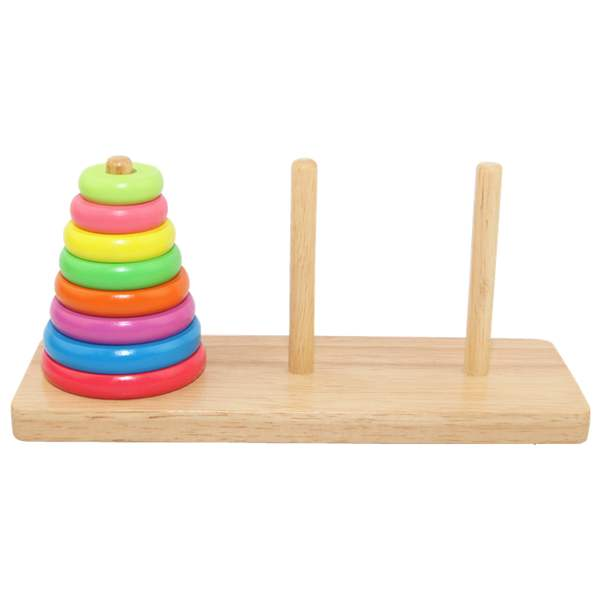
\includegraphics[scale=0.4]{img/C11/11-3/1.png}
    \caption{汉诺塔}
\end{figure}

递归算法求解汉诺塔问题:

\begin{enumerate}
    \item 将前n - 1个圆盘从A柱借助于C柱搬到B柱。
    \item 将最后一个圆盘直接从A柱搬到C柱。
    \item 将n - 1个圆盘从B柱借助于A柱搬到C柱。
\end{enumerate}

\vspace{0.5cm}

\mybox{汉诺塔}

\begin{lstlisting}[language=Python]
def hanoi(n, A, B, C):
    if n == 1
        move(1, A, C)
    else
        hanoi(n-1, A, C, B)
        move(n, A, C)
        hanoi(n-1, B, A, C)
\end{lstlisting}

当圆盘数为64时,假设每次移动花费1秒,总共大约需要5800亿年。 \\

汉诺塔递归算法的递推公式:

\vspace{-0.5cm}

\begin{align*}
    T(n) = \begin{cases}
        1             & n = 1 \\
        2T(n - 1) + 1 & n > 1
    \end{cases}
\end{align*}

利用迭代法,不断用递推方程的右部替换左部,直到出现初值停止迭代。

\vspace{-0.5cm}

\begin{align*}
    T(n) & = 2 * T(n - 1) + 1                     \\
         & = 2 * [ 2 * T(n - 2) + 1] + 1          \\
         & = 2 * [2 * [2 * T(n - 3) + 1] + 1] + 1 \\
         & = \dots                                \\
         & = 2^k * T(n - k) + 2^k - 1             \\
    \\
         & \because n - k = 1                     \\
         & \therefore k = n - 1                   \\
    \\
    T(n) & = 2^{n-1} * T(1) + 2^{n-1} - 1         \\
         & = 2^{n-1} + 2^{n-1} - 1                \\
         & = 2^n - 1                              \\
         & = O(2^n)
\end{align*}

\begin{figure}[H]
    \centering
    
\includegraphics[]{img/C11/11-3/2.png}
\end{figure}

\subsection{插入排序}

插入排序的递推公式: